\documentclass[a4paper,11pt]{article}
	 \usepackage[a4paper, left=2.5cm, bottom=2.5cm]{geometry}
     \usepackage[italian]{babel}
     \usepackage[utf8]{inputenc}
     \usepackage{siunitx}
     \usepackage{graphicx}
     \usepackage{amsfonts}
     \title{Complementi di meccanica classica e termodinamica}
     \author{Appunti vari}
	\date{\today}	

\begin{document}
	\maketitle
\tableofcontents
\newpage

\section{Schifezze utili}
\subsection{Derivata parziale}
Sia $f(x_1,x_2,\cdots,x_n)$ una funzione in più variabili. La derivata parziale rispetto a $x_j$ è
$$\frac{\partial f}{\partial x_j}=\lim\limits_{h\to0}\frac{f(x_1,\cdots,x_j+h,\cdots,x_n)-f(x_1,\cdots,,x_j,\cdots,x_n)}{h}$$
\subsection{Derivata totale}

Sia $f(x_1,x_2,\cdots,x_n,t)$ una funzione in più variabili, allora la derivata totale è
$$\frac{\mathrm{d}f}{\mathrm{d}t}=\frac{\partial f}{\partial t}+\sum_{i=1}^{n}\frac{\partial f}{\partial x_i}\dot{x}_i$$
\subsection{Relazioni tra derivate}

\noindent La derivata totale e la derivata parziale commutano, infatti
$$\frac{\mathrm{d}}{\mathrm{d}t}\frac{\partial f}{\partial x_j}=\sum_{i=1}^{n}\frac{\partial^2 f}{\partial x_i \partial x_j}\dot{x}_i+\frac{\partial^2 f}{\partial t \partial x_j}=\frac{\partial}{\partial x_j}\left(\sum_{i=1}^{n}\frac{\partial f}{\partial x_i}\dot{x}_i+\frac{\partial f}{\partial t}\right)=\frac{\partial \dot{f}}{\partial x_j}$$

\subsection{Campi}

\noindent Un campo scalare è una funzione del tipo $V=V(x,y,z)$. Un campo vettoriale è una funzione del tipo $\vec{F}=(F_x(x,y,z),F_y(x,y,z),F_z(x,y,z))$. Inoltre, un campo vettoriale ruota come un vettore.

\subsection{Operatori}

\noindent Si definisce gradiente di un campo scalare il vettore $$\vec{\nabla}V=\left(\frac{\partial V}{\partial x},\frac{\partial V}{\partial y},\frac{\partial V}{\partial z} \right)$$
Si definisce divergenza di un campo vettoriale lo scalare
$$\vec{\nabla}\cdot\vec{F}=\frac{\partial F_x}{\partial x}+\frac{\partial F_y}{\partial y}+\frac{\partial F_z}{\partial z}$$
Si definisce rotore di un campo vettoriale il vettore
$$\vec{\nabla}\times\vec{F}=\varepsilon_{ijk}\frac{\partial F_k}{\partial x_j}\hat{x}_i$$
\subsection{Integrali}

\noindent Si definisce integrale di linea di un campo vettoriale lungo la curva $\gamma$ l'integrale
$$\int_{\gamma}\vec{F}\cdot\mathrm{d}\vec{r}$$
Si definisce flusso di un campo vettoriale attraverso la superficie $S$ l'integrale
$$\int_{S}\vec{F}\cdot\mathrm{d}\vec{A}$$
\subsection{Teoremi vari}

\noindent Valgono il teorema di Gauss
$$\int_{\partial V}\vec{F}\cdot\mathrm{d}\vec{A}=\int_{V}\vec{\nabla}\cdot\vec{F}\mathrm{d}V$$
e il teorema di Stokes
$$\oint_{\partial S}\vec{F}\cdot\mathrm{d}\vec{r}=\int_{S}\vec{\nabla}\times\vec{F}\cdot\mathrm{d}\vec{A}$$

\subsection{Identità vettoriali ricorrenti}
\[\nabla\cdot\nabla f=\nabla^2f\]
\[\nabla\times\nabla f=0\]
\[\nabla\cdot\nabla\times\vec{v}=0\]
\[\nabla\times(\nabla\times\vec{v})=-\nabla^2\vec{v}+\nabla(\nabla\cdot\vec{v})\]
\[\frac{1}{2}\nabla\vec{v}^2=\vec{v}\times(\nabla\times\vec{v})+(\vec{v}\cdot\nabla)\vec{v}\]
\newpage
\section{Energia}
Se il lavoro della forza non dipende dalla traiettoria, ma unicamente dai punti iniziale e finale, la forza si dice conservativa e posso definire un potenziale. Se $\vec{r}_0$ è un punto qualunque dello spazio, ho
$$U(\vec{r})=-\int_{\vec{r}_0}^{\vec{r}}\vec{F}\cdot\mathrm{d}\vec{r}$$
e ottengo $\vec{F}(\vec{r})=-\vec{\nabla}U(\vec{r})$. Notiamo che la conservatività implica
$$\oint_{\gamma}\vec{F}\cdot\mathrm{d}\vec{r}=0$$
Su una qualunque curva chiusa $\gamma$. Allora, per il teorema di Stokes, la conservatività di $\vec{F}$ è equivalente alla condizione $\vec{\nabla}\times\vec{F}=0$ (a parte schifezze tipo $1/r^2$ nell'origine).

\subsection{Forze centrali}

\noindent Una forza centrale è del tipo $\vec{F}(\vec{r})=f(r)\hat{r}$. Segue che una forza centrale è sempre conservativa.

\subsection{Punti di equilibrio}

\noindent Un punto $\vec{r}_0$ dello spazio è di equilibrio per $\vec{F}(\vec{r})$ se e solo se $\vec{\nabla}U(\vec{r}_0)=~0$. Allora, espandendo il potenziale al secondo ordine, ottengo una forma quadratica

$$U(x,y,z)\approx U(x_0,y_0,z_0)+\frac{1}{2}\left.\frac{\partial^2U}{\partial x^2}\right|_{x_0,y_0,z_0}(x-x_0)^2+\left.\frac{1}{2}\frac{\partial^2U}{\partial y^2}\right|_{x_0,y_0,z_0}(y-y_0)^2+$$
$$+\left.\frac{1}{2}\frac{\partial^2U}{\partial z^2}\right|_{x_0,y_0,z_0}(z-z_0)^2+\left.\frac{\partial^2U}{\partial x\partial y}\right|_{x_0,y_0,z_0}(x-x_0)(y-y_0)+$$ $$+\left.\frac{\partial^2U}{\partial x\partial z}\right|_{x_0,y_0,z_0}(x-x_0)(z-z_0)+\left.\frac{\partial^2U}{\partial y\partial z}\right|_{x_0,y_0,z_0}(y-y_0)(z-z_0)$$
Da qui in poi posso giocare un po' come mi pare con i modi normali.

\newpage
\section{Lagrangiana}
Definiamo lagrangiana di un sistema fisico la quantità
$$\mathcal{L}=T-V$$
dove $T$ è l'energia cinetica e $V$ l'energia potenziale.
\subsection{Equazioni di Eulero-Lagrange}
Vale il principio di minima azione, ovvero la traiettoria seguita da un corpo è un estremale per l'azione $\mathcal{S}$, definita come
$$\mathcal{S}=\int_{t_1}^{t_2}\mathcal{L}(q,\dot{q}, t)\mathrm{d}t$$
Da ciò si deduce (cfr. Landau, Lifshitz, \textit{Mechanics}, cap. 1) che devono valere le equazioni di Eulero-Lagrange
$$\frac{\mathrm{d}}{\mathrm{d}t}\frac{\partial\mathcal{L}}{\partial\dot{x}_j}=\frac{\partial\mathcal{L}}{\partial x_j}$$
Infatti, se $\mathcal{S}$ ha un valore estremale per $q(t)$, allora la trasformazione $q_1(t)=q(t)+\varepsilon(t)$, con $\varepsilon(t_1)=\varepsilon(t_2)=0$, non produce variazioni al prim'ordine in $\mathcal{S}$. Allora deve essere
$$\Delta\mathcal{S}=\int_{t_1}^{t_2}\left[\mathcal{L}(q+\varepsilon,\dot{q}+\dot{\varepsilon}, t)-\mathcal{L}(q,\dot{q}, t)\right]\mathrm{d}t=0$$
Ciò significa
$$\Delta\mathcal{S}=\int_{t_1}^{t_2}\left(\frac{\partial\mathcal{L}}{\partial q}\varepsilon+\frac{\partial \mathcal{L}}{\partial\dot{q}}\dot{\varepsilon}\right)\mathrm{d}t=\int_{t_1}^{t_2}\varepsilon\left(\frac{\partial\mathcal{L}}{\partial q}-\frac{\mathrm{d}}{\mathrm{d}t}\frac{\partial \mathcal{L}}{\partial\dot{q}}\right)\mathrm{d}t=0$$
Dove si è integrato per parti l'ultimo fattore. Imponendo che l'integrando sia nullo per ogni $\varepsilon$, si ottengono le \textit{E-L}.
\subsection{Cambio di coordinate}

\textbf{\large Teorema} \textit{Se le E-L valgono per un sistema di coordinate (e banalmente per le cartesiane sono equivalenti a $\vec{F}=m\vec{a}$), allora valgono per ogni sistema di coordinate.}\\
\textbf{Dimostrazione}
\noindent Se le nostre coordinate $x_1,\cdots,x_n$ sono cartesiane, allora $\mathcal{L}=\frac{1}{2}m\sum_{i=1}^{n}\dot{x}_i^2-V(x_1,\cdots,x_n)$ e le E-L ci danno $m\ddot{x}_i=-\frac{\partial V}{\partial x_i}$, ovvero la seconda legge di Newton.

\noindent Supponiamo ora che le E-L valgano per il sistema $(x_1,\cdots,x_m)$ e supponiamo di avere un altro sistema $(y_1,\cdots,y_n)$, con $y_j=y_j(x_1,\cdots,x_m)$. In generale, sarà possibile trovare $x_i=x_i(y_1,\cdots, y_n)$. Calcoliamo tante derivate:
$$\frac{\partial\dot{x}_i}{\partial\dot{y}_j}=\frac{\partial}{\partial\dot{y}_j}\left(\sum_{j=1}^{n}\frac{\partial x_i}{\partial y_j}\dot{y}_j+\frac{\partial x_i}{\partial t}\right)=\frac{\partial x_i}{\partial y_j}$$ $$\frac{\partial\mathcal{L}}{\partial\dot{y}_j}=\sum_{i=1}^{n}\frac{\partial\mathcal{L}}{\partial\dot{x}_i}\frac{\partial\dot{x}_i}{\partial\dot{y}_j}$$ $$ \frac{\mathrm{d}}{\mathrm{d}t}\frac{\partial\mathcal{L}}{\partial\dot{y}_j}=\frac{\mathrm{d}}{\mathrm{d}t}\left(\sum_{i=1}^{n}\frac{\partial\mathcal{L}}{\partial\dot{x}_i}\frac{\partial\dot{x}_i}{\partial\dot{y}_j}\right)=$$ $$ =\sum_{i=1}^{n}\left(\frac{\mathrm{d}}{\mathrm{d}t}\left(\frac{\partial\mathcal{L}}{\partial \dot{x}_i}\right)\frac{\partial x_i}{\partial y_j}+\frac{\partial\mathcal{L}}{\partial \dot{x}_i}\frac{\mathrm{d}}{\mathrm{d}t}\left(\frac{\partial x_i}{\partial y_j}\right)\right)=$$ $$=\sum_{i=1}^{n}\left(\frac{\partial\mathcal{L}}{\partial x_i}\frac{\partial x_i}{\partial y_j}+\frac{\partial\mathcal{L}}{\partial\dot{x}_i}\frac{\partial\dot{x}_i}{\partial y_j}\right)=$$ $$=\frac{\partial\mathcal{L}}{\partial y_j}$$
\subsection{Conservazioni}
Supponiamo che la lagrangiana non dipenda esplicitamente da una coordinata $q_k$. Allora otteniamo la legge di conservazione
$\frac{\mathrm{d}}{\mathrm{d}t}\frac{\partial\mathcal{L}}{\partial\dot{q}_k}=0$.
La quantità $\partial\mathcal{L}/\partial\dot{q}_k$ si chiama \textit{momento generalizzato} della coordinata $q_k$ (ma non ha necessariamente le dimensioni di una quantità di moto).

\subsubsection{Conservazione dell'energia}

\noindent Osserviamo che in generale possiamo scrivere l'energia cinetica come
$$T=\frac{1}{2}\sum_{i=1}^{n}\frac{\partial\mathcal{L}}{\partial\dot{q}_i}\dot{q}_i$$
Da cui l'energia si scrive come
$$E=T+V=2T-\mathcal{L}=\sum_{i=1}^{n}\frac{\partial\mathcal{L}}{\partial\dot{q}_i}\dot{q}_i-\mathcal{L}$$
Allora
$$\frac{\mathrm{d}E}{\mathrm{d}t}=\frac{\mathrm{d}}{\mathrm{d}t}\left(\sum_{i=1}^{n}\frac{\partial\mathcal{L}}{\partial\dot{q}_i}\dot{q}_i-\mathcal{L}\right)=$$
$$=\sum_{i=1}^{n}\left(\dot{q}_i\frac{\mathrm{d}}{\mathrm{d}t}\frac{\partial\mathcal{L}}{\partial\dot{q}_i}+\frac{\partial\mathcal{L}}{\partial\dot{q}_i}\ddot{q}_i\right)-\frac{\mathrm{d}\mathcal{L}}{\mathrm{d}t}= $$
$$=\sum_{i=1}^{n}\left(\dot{q}_i\frac{\mathrm{d}}{\mathrm{d}t}\frac{\partial\mathcal{L}}{\partial\dot{q}_i}+\frac{\partial\mathcal{L}}{\partial\dot{q}_i}\ddot{q}_i\right)-$$
$$-\left(\sum_{i=1}^{n}\frac{\partial\mathcal{L}}{\partial q_i}\dot{q}_i+\sum_{i=1}^{n}\frac{\partial\mathcal{L}}{\partial \dot{q}_i}\ddot{q}_i+\frac{\partial\mathcal{L}}{\partial t}\right)=$$$$=-\frac{\partial\mathcal{L}}{\partial t}$$
Ciò significa che $E$ si conserva se e solo se $\mathcal{L}$ non dipende esplicitamente dal tempo, ovvero se la lagrangiana è invariante per traslazioni temporali.
\subsubsection{Altre conservazioni}

\noindent La conservazione della quantità di moto si ha se $\mathcal{L}$ è invariante per traslazioni spaziali, mentre la conservazione del momento angolare si ha se $\mathcal{L}$ è invariante per rotazioni.

\subsubsection{Teorema di Noether} \textit{Ad ogni simmetria della lagrangiana corrisponde una quantità conservata.}

\noindent\textbf{Dimostrazione} Con simmetria di $\mathcal{L}$ intendiamo che se le coordinate variano di una piccola quantità, $\mathcal{L}$ non varia al prim'ordine.
Sia quindi una trasformazione infinitesima delle coordinate rappresentata da una funzione del tipo
$$q_i\mapsto q_i+\varepsilon K_i(q)$$
Ovvero la trasformazione infinitesima da $q$ a $q+\varepsilon K(q)$. L'invarianza della lagrangiana al prim'ordine si scrive come $\partial\mathcal{L}/\partial\varepsilon=0$, ovvero
$$\sum_{i=1}^{n}\left(\frac{\partial\mathcal{L}}{\partial q_i}\frac{\partial q_i}{\partial\varepsilon}+\frac{\partial\mathcal{L}}{\partial \dot{q}_i}\frac{\partial \dot{q}_i}{\partial\varepsilon}\right)=\sum_{i=1}^{n}\left(\frac{\partial\mathcal{L}}{\partial q_i}K_i+\frac{\partial\mathcal{L}}{\partial \dot{q}_i}\dot{K}_i\right)=$$
$$\sum_{i=1}^{n}\left(K_i\frac{\mathrm{d}}{\mathrm{d}t}\frac{\partial\mathcal{L}}{\partial \dot{q}_i}+\frac{\partial\mathcal{L}}{\partial \dot{q}_i}\dot{K}_i\right)=\frac{\mathrm{d}}{\mathrm{d}t}\left(\sum_{i=1}^{n}\frac{\partial\mathcal{L}}{\partial\dot{q}_i}K_i\right)=0$$
Ovvero la quantità
$$P(q,\dot{q})=\sum_{i=1}^{n}\frac{\partial\mathcal{L}}{\partial\dot{q}_i}K_i$$
non varia nel tempo. $P(q, \dot{q})$ si chiama \textit{momento conservato}.

\newpage
\section{Forze centrali}
\subsection{Problema dei due corpi in un potenziale centrale}
\noindent Consideriamo due corpi nello spazio, di massa $m_1$ e $m_2$ e posizione $\vec{r}_1$ e $\vec{r}_2$, soggetti a un potenziale $V(r)$ che dipende solamente dalla loro distanza reciproca $\vec{r}=\vec{r}_1-\vec{r_2}$. La lagrangiana è
$$\mathcal{L}=\frac{1}{2}m_1\dot{\vec{r}}_1^2+\frac{1}{2}m_2\dot{\vec{r}}_2^2-V(r)$$
Poniamo  $M=m_1+m_2$, $\mu=m_1m_2/M$, $\vec{R}=(m_1\vec{r}_1+m_2\vec{r}_2)/M$, ottenendo
$$\mathcal{L}=\frac{1}{2}M\dot{\vec{R}}^2+\frac{1}{2}\mu\dot{\vec{r}}^2-V(r)$$
La coordinata $\vec{R}$ è ciclica, pertanto ottengo la conservazione della posizione del centro di massa, e posso scegliere $\dot{\vec{R}}=0$. Scegliendo le coordinate sferiche, la lagrangiana si riscrive come
$$\mathcal{L}=\frac{1}{2}\mu(\dot{r}^2+r^2\dot{\theta}^2+r^2\sin^2\theta\dot{\phi}^2)-V(r)$$
Di nuovo, $\phi$ è ciclica, pertanto si conserva la quantità $\mu r^2\sin^2\theta\dot{\phi}$, ovvero la componente del momento angolare lungo $\hat{z}$. In realtà, $\vec{L}$ si conserva interamente, dunque istante per istante il piano perpendicolare ad esso è il piano in cui giacciono i raggi vettori e le velocità dei due corpi. Spostandosi in tale sistema di riferimento, centrato nel baricentro, e usando $r$ e $\phi$ come coordinate polari, otteniamo dalle E-L
$$\mu\ddot{r}=\frac{L^2}{\mu r^3}-\frac{\partial V(r)}{\partial r}=-\frac{\partial}{\partial r}\left(\frac{L^2}{2\mu r^2}+V(r)\right)=-\frac{\partial V_{eff}(r)}{\partial r}$$
dove si è usato $L=\mu r^2\dot{\phi}$. Ci siamo dunque ridotti allo studio di un moto unidimensionale di un corpo di massa $\mu$. 
\subsubsection{Orbita in un potenziale gravitazionale}
Facciamo un paio di conti. Posto $u=1/r$:
$$\dot{r}=\frac{\partial r}{\partial \phi}\dot{\phi}=\frac{\partial r}{\partial\phi}\frac{L}{\mu r^2}=-\frac{L}{\mu}\frac{\partial u}{\partial\phi}$$
$$\ddot{r}=-\left(\frac{Lu}{\mu}\right)^2\frac{\partial^2u}{\partial\phi^2}$$
$$\left(\frac{Lu}{\mu}\right)^2\frac{\partial^2u}{\partial\phi^2}=-\frac{L^2u^3}{\mu}+\frac{\partial V(r)}{\partial r}$$
$$\frac{\partial^2u}{\partial\phi^2}+u=\frac{\mu r^2}{L^2}\frac{\partial V(r)}{\partial r}=-\frac{\mu}{L^2}\frac{\partial V(1/u)}{\partial u}$$
Se il potenziale è di tipo gravitazionale, allora $\partial V(r)/\partial r=(Gm_1m_2)/r^2$, da cui si ottiene facilmente
$$\frac{1}{r}=A\cos(\phi+\phi_0)+\frac{G\mu^2M}{L^2}$$
La costante $\phi_0$ è in realtà ininfluente (corrisponde a una rotazione degli assi: scegliere $\phi_0=0$ significa orientare gli assi in modo che il punto di minimo avvicinamento sia su $x$). Notiamo inoltre che $r(\phi)$ non rappresenta l'orbita, ma la distanza reciproca tra i due corpi. Inoltre, fissati $E$ e $L$, i punti di massimo e minimo avvicinamento soddisfano l'equazione 
$$u^2-2u_0u=\frac{2\mu E}{L^2}$$
dove si è posto $u_0=G\mu^2M/L^2$, che corrisponde a un'orbita circolare. Le soluzioni sono
$$\frac{1}{r_{\mp}}=u_0\left(1\pm\sqrt{1+\frac{2\mu E}{L^2}}\right)=u_0\left(1\pm\sqrt{1-\frac{E}{E_0}}\right)$$
E notiamo che per $E\geq0$, $r_+\to+\infty$, ovvero l'orbita è illimitata. Inoltre, per $E>0$ non tutti i valori di $\phi$ sono permessi. La costante $\varepsilon=\sqrt{1-E/E_0}$ è l'eccentricità dell'orbita, pertanto in generale vale
$$r=\frac{r_0}{1-\varepsilon\cos\phi}$$
\subsubsection{Costanti del moto e parametri orbitali}
Nel caso $M\gg m$, ovvero $\mu\approx m$, detti $a,b,c$ rispettivamente il semiasse maggiore, il semiasse minore e la semidistanza tra i fuochi, valgono le relazioni

	$$a=\frac{r_0}{|\varepsilon^2-1|}$$ 	$$b=\frac{r_0}{\sqrt{|\varepsilon^2-1|}}$$ 
	$$c=\frac{\varepsilon r_0}{|\varepsilon^2-1|}$$  	$$\varepsilon=\frac{c}{a}$$ 
	$$r_0=\frac{b^2}{a}$$ 
	


\noindent In funzione delle costanti del moto $E$ e $L$ otteniamo
$$a=\frac{GMm}{2|E|}$$
$$b=\frac{L}{\sqrt{2m|E|}}$$
$$r_0=\frac{L^2}{GMm^2}$$
$$\varepsilon^2=1+\frac{2EL^2}{G^2M^2m^3}$$
$$E=\pm\frac{GMm}{2a}$$
$$L^2=GMm^2\frac{b^2}{a}$$
Infine, detto $\vec{A}$ il vettore di Lenz
$$\vec{A}=\vec{p}\times\vec{L}-GMm^2\hat{r}$$
$$A=GMm^2\varepsilon$$
\subsubsection{Un approfondimento: le leggi di Keplero}
Le prime due leggi sono state verificate esplicitamente (le orbite limitate sono ellissi e il sole occupa uno dei fuochi, inoltre la velocità areolare è costante, come conseguenza della conservazione di $\vec{L}$), mentre la terza necessita di una correzione. Usando la seconda legge, vale
$$\frac{L}{2m}=\frac{\pi ab}{T}$$
Da cui
$$T^2=\frac{4\pi^2}{G(M+m)}a^3$$
che si riduce alla terza legge per $M\gg m$.

\subsection{Sviluppo del potenziale in multipoli}
Consideriamo un corpo esteso di massa $m$ con baricentro nell'origine. Sia $\rho(\vec{r})$ la sua densità nel punto $\vec{r}$. Allora, in un punto $\vec{R}$ qualunque dello spazio il potenziale $V(\vec{R})$ di una massa $M$ vale
$$V(\vec{R})=-GM\int\rho(\vec{r})\frac{\mathrm{d}V}{|\vec{R}-\vec{r}|}$$
dove si intende che l'integrale è esteso al corpo. Ovviamente, $|\vec{R}-\vec{r}|=\sqrt{R^2+r^2+2\vec{R}\cdot\vec{r}}$, quindi se siamo sufficientemente lontani dal corpo possiamo espandere in Taylor, ottenendo
$$V(\vec{R})\approx-\frac{GMm}{R}+\frac{GM}{R^2}\int\rho(\vec{r})\vec{r}\cdot\vec{R}\mathrm{d}V-\frac{GM}{R^3}\int\rho(\vec{r})\left[3\left(\frac{\vec{r}\cdot\vec{R}}{R}\right)^2-r^2\right]\mathrm{d}V$$
Il primo termine è nullo perchè siamo nel sistema di riferimento del centro di massa, ovvero per la gravità non ci sono effetti di dipolo (come ad esempio con le cariche elettriche).

\noindent Come esempio, in sferiche ottengo i seguenti potenziali:
\begin{itemize}
	\item se pongo due masse $m$ sull'asse $z$ a distanza $d/2$ dall'origine
	$$V_z(R,\theta)=-\frac{2GMm}{R}-\frac{GMmd^2}{4R^3}\left(3\cos^2\theta-1\right)$$
	\item se pongo due masse $m$ sull'asse $x$ a distanza $d/2$ dall'origine
	$$V_x(R,\theta)=-\frac{2GMm}{R}-\frac{GMmd^2}{4R^3}\left(3\sin^2\theta\cos^2\phi-1\right)$$
	\item se pongo due masse $m$ sull'asse $y$ a distanza $d/2$ dall'origine
	$$V_y(R,\theta)=-\frac{2GMm}{R}-\frac{GMmd^2}{4R^3}\left(3\sin^2\theta\sin^2\phi-1\right)$$
\end{itemize}

\noindent Più esplicitamente, si può mostrare che esiste una base ortogonale, chiamata armoniche sferiche, tale che nel punto $\vec{R}$, individuato dalle coordinate sferiche $\theta$ e $\phi$, il potenziale è
$$V(\vec{R})=\sum_{l=0}^{+\infty}\sum_{m=-l}^{l}\frac{4\pi}{2l+1}q_{lm}\frac{y_m(\theta,\phi)}{R^l}$$
\subsection{Forze di marea}
Consideriamo ora la terra come una sfera di raggio $r$ che percorre un'orbita circolare di raggio $R$ intorno al sole. In tale sistema, indicando con $\vec{r}$ il vettore che ha origine nel centro della terra e punta nel punto, il potenziale si scrive come
$$V(r)\approx-\frac{GMm}{R}\left[1-\frac{\vec{R}\cdot\vec{r}}{R^2}+\frac{1}{2}\left(3\left(\frac{\vec{R}\cdot\vec{r}}{R^2}\right)^2-\frac{r^2}{R^2}\right)\right]$$
Ovvero, se teniamo conto dell'accelerazione fittizia otteniamo una forza del tipo
$$\vec{F}\approx\frac{GMm}{R^2}\left(3\frac{\vec{R}\cdot\vec{r}}{R^3}\vec{R}-\frac{\vec{r}}{R}\right)=\frac{GMm}{R^3}\left(\begin{array}{c}
2x \nonumber \\
-y \nonumber \\
-z \nonumber
\end{array}\right)$$

Riprendiamo ora l'espressione di $\vec{F}$ e supponiamo di avere un'asta priva di massa di lunghezza $2d$, che si trova nel piano dell'orbita, alle cui estremità sono fissate due masse $m$ collegate da una molla. Posto $\Omega^2=(GM)/R^3$, la forza agente su una massa è 
$$\vec{F}=-\frac{1}{2}\Omega^2md\left[(3\cos2\theta-1)\hat{r}-3\sin2\theta\hat{\theta}\right]$$
Il momento torcente agente sull'asta è invece
$$\vec{\tau}=-3\Omega^2md^2\sin2\theta\hat{z}$$
Immaginiamo ora che il corpo stia ruotando intorno al proprio centro con velocità angolare $\omega\gg \Omega$, che possiamo assumere pressochè costante. Allora, detto $\Delta r$ lo spostamento di una massa e supponendo $\Delta r\ll d$, otteniamo
$$\Delta\ddot{r}+2\gamma\Delta\dot{r}+\omega_0^2\Delta r=-\frac{1}{2}\Omega^2d\left[3\cos(2\omega t)+1\right]$$
La cui soluzione a regime è
$$\Delta r(t)=-\frac{3\Omega^2d}{2\rho}\cos(2\omega t-\phi)-\frac{d\Omega^2}{2\omega_0^2}$$
Supponendo ora $\omega_0\gg\omega$, risulta $\rho\approx\omega_0^2$ e $\phi\approx\tan\phi\approx\frac{4\gamma\omega}{\omega_0^2}$
In particolare, $\phi\neq0$ e in un ciclo il valor medio del modulo di $\vec{\tau}$ è
$$\overline{\tau}=\frac{\omega}{2\pi}\int_{0}^{2\pi/\omega}\tau(t)\mathrm{d}t=-\frac{9\Omega^4m\omega d^2}{2\pi\omega_0^2}\sin\phi$$
Mentre la potenza dissipata è $P=(\vec{F}\cdot\hat{r})\Delta\dot{r}$, con un valor medio in un ciclo di
$$\overline{P}=-9\left(\frac{\Omega}{\omega_0}\right)^4\gamma E$$
Con $E=\frac{1}{2}I\omega^2$. Il tempo caratteristico è quindi
$$t_{lock}=\frac{1}{9\gamma}\left(\frac{\omega_0}{\Omega}\right)^4$$
Dopo un certo numero di tempi caratteristici, il bilanciere sarà in tidal block (ad esempio, il tempo caratteristico della luna è dell'ordine del milione di anni, e in effetti al momento la luna ci mostra sempre la stessa faccia).
\vspace{5mm}

\noindent \textit{N.B.: da qui in poi c'è la parte che Gigi ci ha proposto di far da soli, potrebbero esserci errori. Se li trovate, segnalatemeli.}
\noindent Notiamo che il momento angolare perso nella rotazione aumenta il momento angolare dovuto alla rivoluzione. Infatti, la forza agente del bilanciere in un sistema rotante con origine nel sole e asse $\hat{x}$ che punta verso il pianeta è 
$$\vec{F}=2\Omega^2mR\left[\left(1+\left(\frac{d}{R}\right)^2\left(3\cos^2\theta-1\right)\right)\hat{x}+3\left(\frac{d}{R}\right)^2\sin\theta\cos\theta\hat{y}\right]$$
Ora, dato che $r\ll R$, possiamo supporre che tale forza sia concentrata nel centro di massa del bilanciere, piuttosto che alle due estremità. Ma allora il momento torcente di tale forza è 
$$\vec{\tau}=3\Omega^2md^2\sin2\theta\hat{z}$$
Tra l'altro, il fatto che $\vec{F}\cdot\hat{x}\neq0$ implica che il pianeta si sta pure allontanando dalla stella. A tal proposito, qualcosa di simile sta accadendo al sistema Terra-Luna (il satellite si allontana di circa 1 cm l'anno), ma in questo caso è la Terra a perdere momento angolare. Infatti la sua velocità angolare di rotazione intorno al proprio asse è molto maggiore (circa 28 volte) di quella di rivoluzione della Luna intorno alla Terra.
\newpage
\section{Corpo rigido}
\subsection{Matrici di rotazione}
Consideriamo due sistemi di riferimento ortonormali e destrorsi $(\hat{x}_1,\hat{x}_2,\hat{x}_3)$ e $(\hat{x}'_1,\hat{x}'_2,\hat{x}'_3)$ di $\mathbb{R}^3$. Allora, detta $A$ la matrice di rotazione che mi permette di passare dalla prima terna alla seconda, abbiamo
$$\hat{x}'_i=A_{ij}\hat{x}_j$$
$$A=\left(\begin{array}{c c c c c}
\hat{x}'_1\cdot\hat{x}_1 & & \hat{x}'_1\cdot\hat{x}_2 & & \hat{x}'_1\cdot\hat{x}_3 \\
\hat{x}'_2\cdot\hat{x}_1 & &\hat{x}'_2\cdot\hat{x}_2 & & \hat{x}'_2\cdot\hat{x}_3 \\
\hat{x}'_3\cdot\hat{x}_1 & &\hat{x}'_3\cdot\hat{x}_2 & & \hat{x}'_3\cdot\hat{x}_3 \\
\end{array}\right)$$

\noindent Chiaramente $A_{ij}$ è il coseno di un angolo, pertanto i termini di $A$ si chiamano anche coseni direttori, ed è altrettanto chiaro che se $B$ è la matrice che permette di passare dalla seconda terna alla prima, risulta $B=A^t$. Mostriamo ora qualche proprietà delle matrici di rotazione:
\begin{enumerate}
	\item Le colonne e le righe di $A$ sono una base ortonormale per il prodotto scalare canonico. Infatti per le righe risulta $$\delta_{ij}=\hat{x}'_i\cdot\hat{x}'_j=A_{ik}\hat{x}_k\cdot A_{jm}\hat{x}_m=A_{ik}A_{jm}\delta_{km}=A_{im}A_{jm}$$
	E in maniera analoga per le colonne passando a $B$.
	\item Segue che $A$ ha solo 3 parametri indipendenti, perchè ha 9 entrate ma 6 vincoli.
	\item $A$ è ortogonale. Infatti $$a^{-1}_{qj}=\delta_{qi}a^{-1}_{ij}=(a_{kq}a_{ki})a^{-1}_{ij}=a_{kq}(a_{ki}a^{-1}_{ij})=a_{kq}\delta_{kj}=a_{jq}$$
	\indent Se $X,X'$ sono i vettori delle coordinate di un vettore rispetto alle due basi, ovviamente $X'=AX$. Allo stesso modo, se $D,D'$ sono le matrici associate a $f\in\mathcal{L}(\mathbb{R}^3)$ rispetto alle due basi, $D'=ADA^{-1}$.
	\item $\det A=1$, infatti $$1=\det I=\det(AA^{-1})=\det A\det A^{-1}=\det A\det A^t=(\det A)^2$$ e il segno meno va scartato perchè rappresenta una riflessione.
	\item L'unico autovalore reale è 1, quindi se $\Omega$ è l'angolo di rotazione esiste una base in cui essa è rappresentata dalla matrice
	$$\left(\begin{array}{c c c c c}
	\cos\Omega & & \sin\Omega & & 0 \\
	-\sin\Omega & & \cos\Omega & & 0 \\
	0 & & 0 & & 1 \\
	\end{array}\right)$$
	mentre su $\mathbb{C}$ ci sono anche gli autovalori $e^{\pm i\Omega}$. 
\end{enumerate}
\subsection{Angoli di Eulero}
Eulero ebbe la brillante idea di rappresentare le rotazioni nel seguente e utilissimo modo:
\begin{itemize}
	\item dal sistema $(\hat{X},\hat{Y},\hat{Z})$ si passa al sistema $(\hat{\xi},\hat{\upsilon},\hat{\zeta})$ tramite una rotazione di $\phi$ intorno a $\hat{Z}$,
	\item dal sistema $(\hat{\xi},\hat{\upsilon},\hat{\zeta})$ si passa al sistema $(\hat{\xi}',\hat{\upsilon}',\hat{\zeta}')$ tramite una rotazione di $\theta$ intorno a $\hat{\xi}$,
	\item infine dal sistema $(\hat{\xi}',\hat{\upsilon}',\hat{\zeta}')$ si passa al sistema $(\hat{x}_1,\hat{x}_2,\hat{x}_3)$ tramite una rotazione di $\psi$ intorno a $\hat{\zeta}'$.
\end{itemize}
\vspace{5mm}
In tal modo otteniamo la splendida matrice di rotazione
$$\left(\begin{array}{c c c c c}
\cos\psi\cos\phi-\cos\theta\sin\phi\sin\psi && \cos\psi\sin\phi+\cos\theta\cos\phi\sin\psi && \sin\psi\sin\theta \\
-\sin\psi\cos\phi-\cos\theta\sin\phi\cos\psi && -\sin\psi\sin\phi+\cos\theta\cos\phi\cos\psi && \cos\psi\sin\theta \\
\sin\theta\sin\phi && -\sin\theta\cos\phi && \cos\theta \\
\end{array}\right)$$
E dato che la traccia è invariante per similitudine, otteniamo 
$$\cos\frac{\Omega}{2}=\cos\frac{\theta}{2}\cos\frac{\phi+\psi}{2}$$
In generale, se la matrice $A$ rappresenta una rotazione infinitesima, si può scrivere come
\[A=\mathbb{I}+\left(\begin{array}{c c c}
0 & \mathrm{d}\theta+\mathrm{d}\psi & 0 \\
-\mathrm{d}\theta-\mathrm{d}\psi & 0 & \mathrm{d}\theta \\
0 & -\mathrm{d}\theta & 0 
\end{array}\right)=\mathbb{I}+\mathrm{d}\Omega\left(\begin{array}{c c c}
0 & n_3 & -n_2 \\
-n_3 & 0 & n_1 \\
n_2 & -n_1 & 0 
\end{array}\right)\]
Dove $\mathrm{d}\Omega$ rappresenta l'ampiezza dell'angolo di rotazione intorno al versore $\hat{n}=n_1\hat{x}+~n_2\hat{y}+~n_3\hat{z}$. 

\begin{figure}
	\centering
	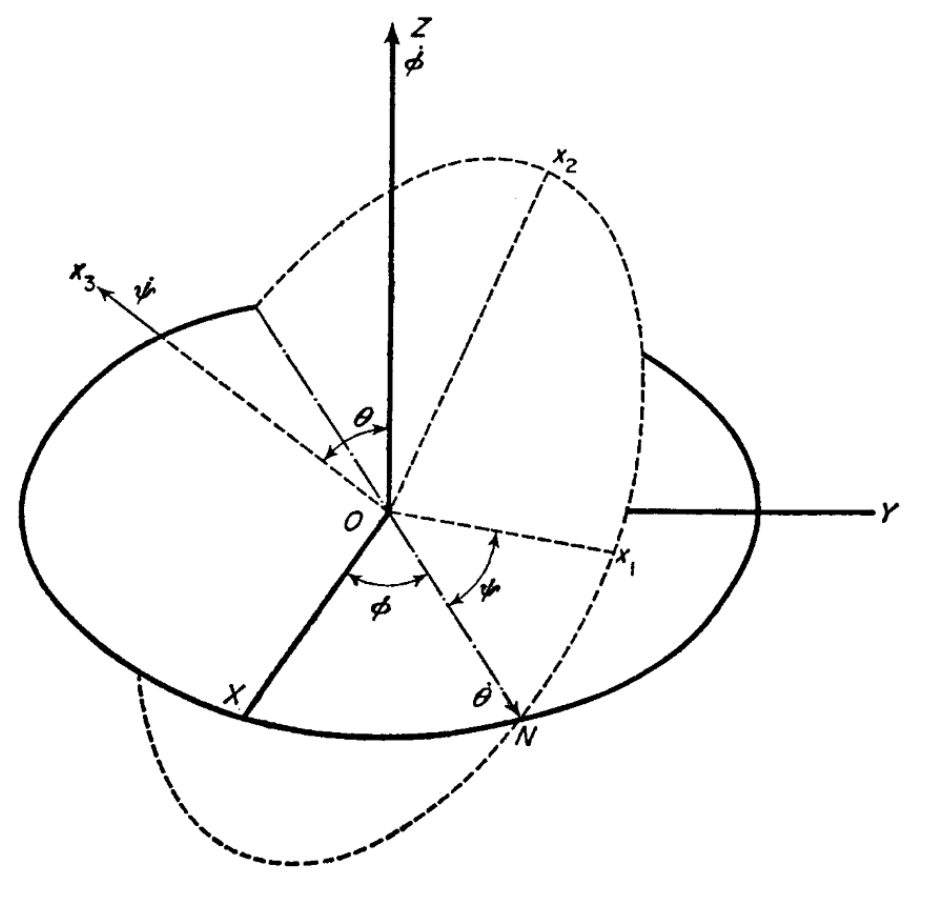
\includegraphics[scale=0.37]{angoli_eulero.png}
	\caption{\textit{Angoli brutti}\label{Eulero}}
\end{figure}

\subsection{Moto di un corpo rigido}

Lo pseudovettore $\vec{\omega}=\hat{n}\frac{\mathrm{d}\Omega}{\mathrm{d}t}$ rappresenta la velocità angolare del corpo intorno all'asse $\hat{n}$. Sappiamo ora che, fissato un punto $P$ la cui posizione è $\vec{r}_P$, la posizione di qualunque altro punto $Q$ è
\[\vec{r}_Q=\vec{r}_P+\vec{r}_{PQ}\]
dove $\vec{r}_{PQ}$ è il vettore con coda in $P$ e punta in $Q$. Derivando e usando il teorema di Poisson, e ricordando che il corpo è rigido, otteniamo
\[\dot{\vec{r}}_Q=\dot{\vec{r}}_P+\vec \omega_P\times\vec{r}_{PQ}\]
Ovvero il moto del corpo rigido è la composizione di una traslazione e di una rotazione. 

\noindent Mostriamo che la velocità angolare è la stessa, qualunque sia $P$. Siano dunque $P_1$, $P_2$ due punti del corpo rigido nelle posizioni $\vec{r}_1$ e $\vec{r}_2$ e sia $\vec{r}=\vec{r}_2-\vec{r}_1$. Allora, dette $\vec \omega_1$ e $\vec \omega_2$ le velocità angolari relative a $P_1$ e $P_2$, abbiamo 
\[\dot{\vec{r}}_2=\dot{\vec{r}}_1+\vec{\omega}_1\times\vec{r}\]
\[\dot{\vec{r}}_1=\dot{\vec{r}}_2-\vec{\omega}_2\times\vec{r}\]
Ovvero
\[\left(\vec{\omega}_1-\vec{\omega}_2\right)\times\vec{r}=0\]
Preso ora $Q$ di posizione $\vec{r}_Q$, si ha
\[\dot{\vec{r}}_1+\vec{\omega}_1\times\left(\vec{r}_Q-\vec{r}_1\right)=\dot{\vec{r}}_2+\vec{\omega}_2\times\left(\vec{r}_Q-\vec{r}_2\right)\]
Svolgendo i calcoli, si trova
\[\left(\vec{\omega}_1-\vec{\omega}_2\right)\times\vec{r}_Q=0\]
Per l'arbitrarietà di $Q$, le due velocità angolari sono uguali. Allora per l'arbitrarietà di $P_1$ e $P_2$, la velocità angolare è la stessa per tutti i punti del corpo. Da ciò si ottiene il

\noindent\textbf{Teorema di Eulero:} \textit{il moto di un corpo rigido di cui esiste un punto fermo è una pura rotazione intorno a un certo asse.}

\noindent Sia infatti $P$ tale punto. Allora per un generico punto $Q$ la velocità si scrive come
\[\vec{v}_Q=\vec{\omega}\times(\vec{r}_Q-\vec{r}_P)\]
che rappresenta chiaramente una rotazione intorno all'asse istantaneo individuato dai punti sulla retta parallela a $\vec{\omega}$ e passante per $P$.


\subsection{Tensore di inerzia}
Consideriamo un corpo rigido formato da una collezione $P_1,P_2,\cdots,P_n$ di punti materiali di posizione $\vec{r}_1,\vec{r}_2,\cdots,\vec{r}_n$ e di massa $m_1,m_2,\cdots,m_n$ (la generalizzazione al corpo continuo è immediata scambiando integrali con sommatorie). Il momento angolare del corpo è
\[\vec{L}=\sum_{\alpha=1}^{n}m_{\alpha}\vec{r}_\alpha\times\left(\vec \omega\times\vec{r}_\alpha\right)\]
Svolgendo i calcoli, si ottiene
\[L_i=I_{ij}\omega_j\]
Con
\[I_{ij}=\sum_{\alpha=1}^{n}m_\alpha\left(r^2_{\alpha}\delta_{ij}-r_{i,\alpha}r_{j,\alpha}\right)\]
Il tensore $I$ prende il nome di tensore di inerzia e, udite udite, ha la splendida proprietà di ruotare come un tensore!

\noindent L'energia cinetica del corpo è banalmente
\[T=\frac{1}{2}\sum_{\alpha=1}^{n}m_\alpha v^2_\alpha=\frac{1}{2}\sum_{\alpha=1}^{n}m_\alpha \left(\vec{\omega}\times\vec{r}_\alpha \right)\cdot\vec{v}_\alpha=\frac{1}{2}\vec{L}\cdot\vec{\omega}=\frac{1}{2}\vec{\omega}^t\cdot I\vec{\omega}\]
In maniera analoga a quanto visto nel calcolo dell'energia cinetica, per un qualsiasi versore $\hat{n}$ abbiamo la seguente identità
\[\hat{n}\cdot I\hat{n}=\sum_{\alpha=1}^{n}m_\alpha\left(\vec{r}_\alpha\times\hat{n}\right)^2\]
che è il momento di inerzia intorno all'asse passante per $\hat{n}$.

\noindent Inoltre, $I$ è chiaramente simmetrico, dunque per il teorema spettrale esiste una base ortonormale di autovettori. Tale autovettori sono detti assi principali di inerzia e gli autovalori $I_1$, $I_2$, $I_3$ sono detti momenti principali di inerzia.

\subsection{Equazioni di Eulero}
Consideriamo un corpo rigido e un sistema di coordinate solidale con il corpo, con assi coincidenti con gli assi principali. Allora in tale sistema la seconda equazione cardinale si scrive come
\[\frac{\delta \vec{L}}{\delta t}+\vec{\omega}\times\vec{L}=\vec{\tau}\]
Dove $\frac{\delta\vec{L}}{\delta t}=\dot{L}_i\hat{x_i}$, con $\hat{x}_i$ versori del sistema rotante.
Scrivendo tale equazione in componenti otteniamo le equazioni di Eulero
\[I_1\dot{\omega}_1=\omega_2\omega_3\left(I_2-I_3\right)+\tau_1\]
\[I_2\dot{\omega}_2=\omega_3\omega_1\left(I_3-I_1\right)+\tau_2\]
\[I_3\dot{\omega}_3=\omega_1\omega_2\left(I_1-I_2\right)+\tau_3\]

\subsection{Ellissoidi di inerzia e di Binet. Moto libero}
Scegliamo come sistema di coordinate un sistema in cui il tensore di inerzia sia diagonale, con la convenzione $I_1\leq I_2\leq I_3$. Sia $\hat{n}$ un versore e poniamo
\[\vec{\rho}=\frac{\hat{n}}{\sqrt{\hat{n}\cdot I\hat{n}}}\]
In tal modo, detta $\rho_i$ l'$i$-esima componente di $\vec{\rho}$, si ha
\[I_1\rho_1^2+I_2\rho_2^2+I_3\rho_3^2=1\]
ovvero un ellissoide, noto come ellissoide di inerzia. Qualitativamente, la lunghezza del semiasse dell'ellissoide lungo $\hat{x}_j$ sarà grande se $I_j$ è grande e viceversa.

\noindent Notiamo ora che
\[\vec{\rho}=\frac{\omega\hat{n}}{\omega\sqrt{\hat{n}\cdot I\hat{n}}}=\frac{\vec{\omega}}{\sqrt{2T}}\]
Posto
\[f(\vec{\rho})=\rho_i^2 I_{ii}\]
si ha $\left(\nabla f\right)_i=\frac{2L_i}{\sqrt{2T}}$. Dato che il gradiente rappresenta la direzione di massima pendenza e $f(\vec\rho)=1$ rappresenta l'ellissoide di inerzia, $\vec L$ è ortogonale a quest'ultimo. In particolare, se $\vec{L}$ è costante l'ellissoide si muove in modo da mantenere tale ortogonalità, come si vede in figura (\ref{ellissoideinerzia}). Inoltre, dato che
\[\vec{\rho}\cdot\hat{L}=\sqrt{2T}\]
la distanza tra piano tangente e centro dell'ellissoide rimane costante nel tempo. Questa descrizione, nota come costruzione di Poinsot, permette di determinare interamente il moto del corpo, una volta noti $\vec{L}$ e $T$. Infatti, l'orientazione del corpo è la stessa dell'ellissoide di inerzia, e $\vec{\omega}$ è diretta come $\vec{\rho}$.
\begin{figure}
	\centering
	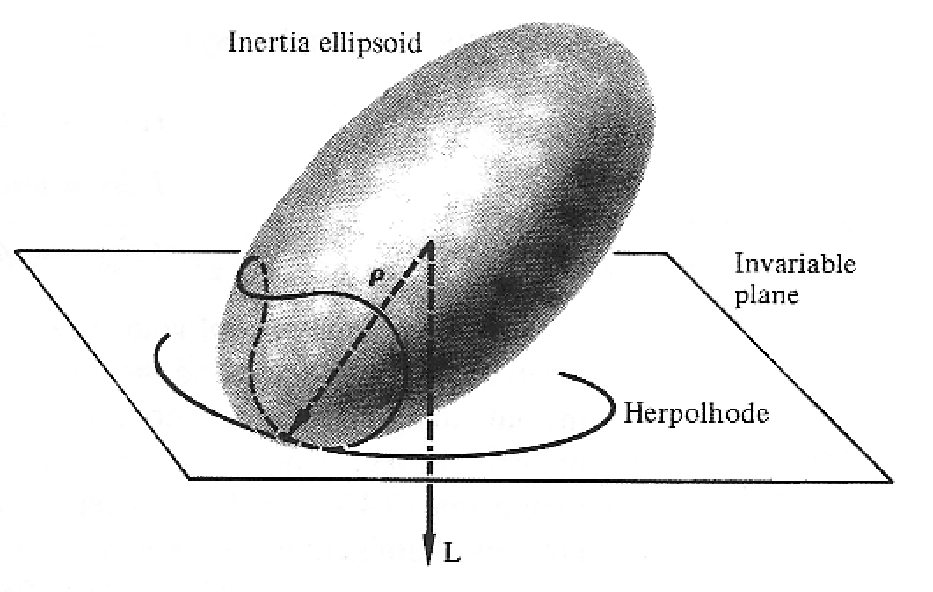
\includegraphics[scale=0.6]{ellissoide_inerzia.png}
	\caption{\textit{Moto dell'ellissoide di inerzia.}}
	\label{ellissoideinerzia}
\end{figure}
\vspace{5mm}

\noindent Se invece ora consideriamo l'energia cinetica e il modulo del momento angolare, otteniamo
\[\left\{\begin{array}{l}
2T=I_1\omega_1^2+I_2\omega_2^2+I_3\omega_3^2 \\
\\
L^2=I_1^2\omega_1^2+I_2^2\omega_2^2+I_3^2\omega_3^2
\end{array}\right.\]
che possiamo riscrivere nella forma
\[\left\{\begin{array}{l}
\frac{L^2_x}{2TI_1}+\frac{L^2_y}{2TI_2}+\frac{L^2_z}{2TI_3}=1 \\
\\
\frac{L^2_x}{L^2}+\frac{L^2_y}{L^2}+\frac{L^2_z}{L^2}=1
\end{array}\right.\]
La prima curva è ancora un ellissoide, chiamato ellissoide di Binet, in cui però l'asse maggiore corrisponde al momento di inerzia minore. Inoltre, si deduce che, fissati $T$ e $L$, l'intersezione tra l'ellissoide di Binet e la sfera di raggio $L$ rappresenta la regione dello spazio delle fasi in cui possono variare le componenti di $\vec{L}$. In particolare, si hanno intersezioni se $\sqrt{2TI_1}\leq~L\leq~\sqrt{2TI_3}$. Una visualizzazione dell'ellissoide di Binet è riportata in figura (\ref{ellissoidebinet}).
\begin{figure}
	\centering
	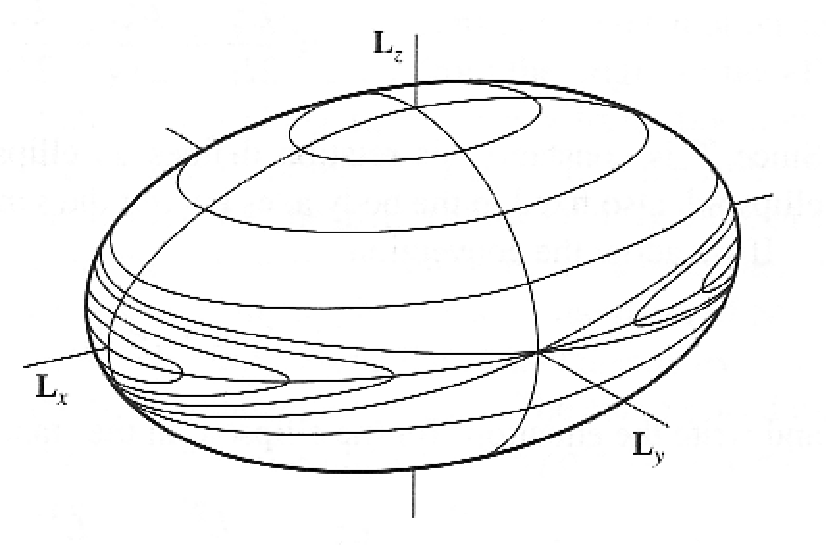
\includegraphics[scale=0.6]{ellissoide_binet.png}
	\caption{\textit{Ellissoide di Binet. Le curve rappresentano le intersezioni con la sfera, ovvero le traiettorie possibili per le componenti di $\vec{L}$.}}
	\label{ellissoidebinet}
\end{figure}
\vspace{5mm}

\noindent Consideriamo come prima un corpo rigido in un sistema di coordinate con assi coincidenti con gli assi principali e tali che $I_1\leq I_2\leq I_3$. Vogliamo studiare la stabilità attorno a uno degli assi. Supponiamo ad esempio $\vec{\omega}=\left(\omega,\varepsilon_2,\varepsilon_3\right)$, con $\varepsilon_i\ll\omega$. Allora le equazioni di Eulero si scrivono come
\[\dot{\omega}\approx0\]
\[I_2\dot{\varepsilon}_2=\varepsilon_3\omega(I_3-I_1)\]
\[I_3\dot{\varepsilon}_3=\varepsilon_2\omega(I_1-I_2)\]
Ipotizzando una soluzione del tipo $\varepsilon_k=A_ke^{\lambda t}$, si ottiene
\[\lambda=\pm\sqrt{\frac{I_3-I_1}{I_2}\frac{I_1-I_2}{I_3}}\]
Chiaramente, se $\lambda\in\mathbb{R}$, $\varepsilon_k$ cresce esponenzialmente e non c'è stabilità. Se invece $\lambda$ è immaginario puro c'è stabilità, perchè $\varepsilon_k$ oscilla intorno allo 0 con ampiezza molto minore di $\omega$. Ma ciò significa che c'è stabilità se $\vec\omega$ è diretta lungo $\hat{x}_1$ o $\hat{x}_3$, come si vede ciclando gli indici.
\subsection{Moto di una trottola}
Consideriamo un corpo in cui due momenti principali di inerzia siano uguali e scegliamo il sistema di coordinate in cui
\[\mathbb{I}=\left(\begin{array}{c c c}
I & 0 & 0 \\
0 & I & 0 \\
0 & 0 & I_3
\end{array}\right)\]
Vogliamo studiare il moto del corpo nel caso in cui quest'ultimo è immerso in un campo gravitazionale costante ed esiste un punto fisso. Utilizzando gli angoli in figura (\ref{trottola}), la lagrangiana del sistema si scrive come
\[\mathcal{L}=\frac{1}{2}I\left(\dot{\theta}^2+\dot{\phi}^2\sin^2\theta\right)+\frac{1}{2}I_3\left(\dot{\psi}+\dot{\phi}\cos\theta\right)^2-Mgl\cos\theta\]
dove $M$ è la massa della trottola e $l$ la distanza tra centro di massa e punto fisso. Notiamo che $\phi$ e $\psi$ sono cicliche, quindi si conservano le quantità
\[P_{\phi}=I\dot{\phi}\sin^2\theta+I_3\cos\theta\left(\dot{\psi}+\dot{\phi}\cos\theta\right)=Ib\]
\[P_{\psi}=I_3\left(\dot{\psi}+\dot{\phi}\cos\theta\right)=Ia\]
dove $a$ e $b$ sono lettere opportune.
Ovviamente una terza costante del moto è l'energia, dato che $\mathcal{L}$ non dipende esplicitamente dal tempo.
\begin{figure}
	\centering
	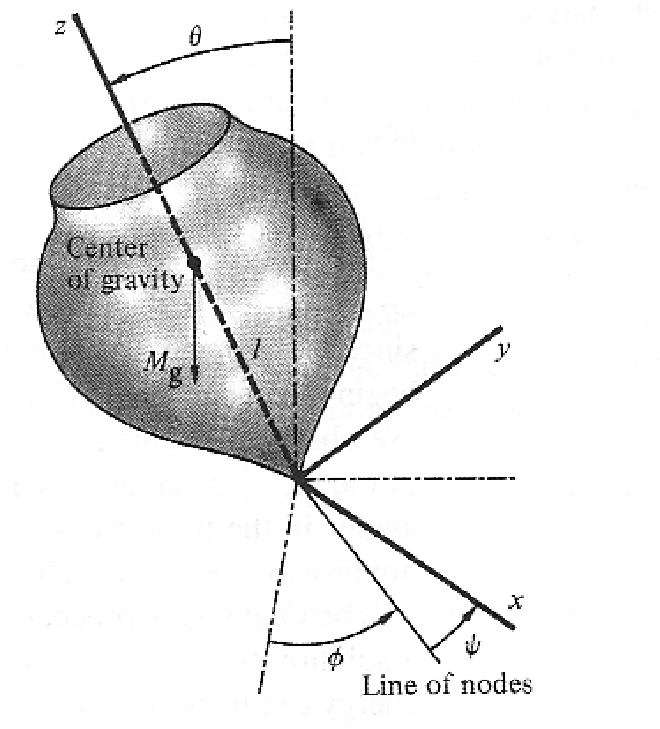
\includegraphics[scale=0.6]{trottola.png}
	\caption{\textit{gli angoli di Eulero usati nello studio del moto della trottola.}}
	\label{trottola}
\end{figure}

\noindent Con le giuste sostituzioni, si arriva all'equazione
\[E=\frac{1}{2}I\dot{\theta}^2+\frac{1}{2}I\left(\frac{b-a\cos\theta}{\sin\theta}\right)^2+\frac{1}{2}\frac{I^2a}{I_3^2}+Mgl\cos\theta\]
che può essere integrata a occhio per dare $\theta(t)$.

\newpage

\section{Esercizi vari}
\subsection{Forze centrali}
\noindent\textbf{Precessione} \textit{Si perturbi il potenziale gravitazionale $U_0$ con una piccola correzione $\delta U$. Dire di quanto precede l'orbita nei seguenti casi:
\begin{itemize}
	\item $\delta U=\beta/r^2$
	\item $\delta U=\gamma/r^3$
\end{itemize}}

\noindent Sia $U_0=-\alpha/r$ il potenziale imperturbato. Nel primo caso, possiamo trovare l'equazione esatta dell'orbita, che risulta
$$r(\theta)=\frac{p}{1+\varepsilon\cos\omega\theta}$$
con 
$$\omega=\sqrt{1+\frac{2m\beta}{L^2}}$$
In tal caso l'orbita precede di 
$\delta\theta=2\pi\left(\frac{1}{\omega}-1\right)$. In generale, dalla conservazione dell'energia e del momento angolare otteniamo
$$\dot{r}^2=\frac{2}{m}\left(E-U-\frac{L^2}{2mr^2}\right)$$
$$\mathrm{d}t=\frac{mr^2}{L}\mathrm{d}\theta$$
L'angolo spazzato in un giro è allora
$$\Delta\theta=2\int_{r_{min}}^{r_{max}}\frac{L}{r^2}\frac{\mathrm{d}r}{\sqrt{\frac{2}{m}\left(E-U\right)-\frac{L^2}{2mr^2}}}=$$
$$=-2\frac{\partial}{\partial L}\int_{r_{min}}^{r_{max}}\sqrt{2m(E-U)-\frac{L^2}{r^2}}\mathrm{d}r$$
Espandendo l'ultima espressione
$$\Delta\theta=-2\frac{\partial}{\partial L}\int_{r_{min}}^{r_{max}}\left(\sqrt{2m(E-U_0)-\frac{L^2}{r^2}}-\frac{m\delta U}{\sqrt{2m(E-U_0)-\frac{L^2}{r^2}}}\right)\mathrm{d}r=$$
$$=2\pi+2\frac{\partial}{\partial L}\int_{r_{min}}^{r_{max}}\frac{m\delta U}{\sqrt{2m(E-U_0)-\frac{L^2}{r^2}}}\mathrm{d}r$$
Otteniamo $$\delta\theta=2\frac{\partial}{\partial L}\int_{r_{min}}^{r_{max}}\frac{m\delta U}{\sqrt{2m(E-U_0)-\frac{L^2}{r^2}}}\mathrm{d}r$$
Nel primo caso otteniamo il risultato precedente espanso al prim'ordine. Nel secondo caso, supponendo che la deviazione dall'orbita non perturbata sia trascurabile, otteniamo
$$\delta\theta=-\frac{6\pi m^2\gamma\alpha}{L^4}$$
\vspace{5mm}

\noindent\textbf{Potenziale repulsivo} \textit{Dato un potenziale repulsivo del tipo $V(r)=k/r$, trovare l'orbita e i suoi parametri in funzione di energia e momento angolare e trovare l'angolo di deflessione per una particella proveniente dall'infinito.}

\noindent Con facili conti si trova
$$r(\theta)=\frac{l}{\varepsilon\cos\theta-1}$$
dove 
$$l=\frac{L^2}{mk}$$
$$\varepsilon=\sqrt{1+\frac{2EL^2}{mk^2}}$$
Banalmente l'angolo di deflessione è $\Delta\phi=\pi-2\arccos\frac{1}{\varepsilon}$.
\vspace{5mm}

\noindent\textbf{Punti lagrangiani} \textit{Trovare i punti sul piano dell'orbita terrestre tali che la risultante delle forze gravitazionali del sistema Terra-Sole permette un'orbita circolare di periodo uguale al periodo di rivoluzione terrestre}

\noindent Scegliamo un sistema di riferimento non inerziale con origine nel baricentro del sistema Terra-Sole che ruota solidalmente con la Terra. Come sistema di coordinate, scegliamo le polari. Tralasciamo i punti sull'asse Terra-Sole, la loro posizione si trova facilmente. Cerchiamo invece i punti con $\theta\neq0$ Allora, detti $M_T,\vec{r}_T, M_S,\vec{r}_S$ le masse e i vettori posizione di Terra e Sole, vale
$$m\ddot{\vec{r}}=-\frac{GM_Sm}{|\vec{r}-\vec{r_S}|^3}(\vec{r}-\vec{r}_S)-\frac{GM_Tm}{|\vec{r}-\vec{r_T}|^3}(\vec{r}-\vec{r}_T)-m\vec{\omega}\times(\vec{\omega}\times\vec{r})$$
dove l'unica forza fittizia è quella centrifuga, dato che nei punti di equilibrio la velocità è nulla (e dunque anche il termine di Coriolis). Imponendo che l'accelerazione sia nulla lungo $\hat{r}$ e $\hat{\theta}$, otteniamo
$$\frac{M_S(r+r_S\cos\theta)}{|\vec{r}-\vec{r}_S|^3}+\frac{M_T(r-r_T\cos\theta)}{|\vec{r}-\vec{r}_T|^3}=\frac{\omega^2r}{G}$$
$$\frac{M_Sr_S\sin\theta}{|\vec{r}-\vec{r}_S|^3}=\frac{M_Tr_T\sin\theta}{|\vec{r}-\vec{r}_T|^3}$$
Abbiamo supposto $\theta\neq0$, e poichè siamo nel sistema del centro di massa vale $M_Sr_S=M_Tr_T$. Allora l'ultima equazione ci dà $|\vec{r}-\vec{r}_S|=|\vec{r}-\vec{r}_T|=d$, ovvero il corpo si trova sull'asse della congiungente Terra-Sole. Inserendo questo risultato nella prima otteniamo
$$d=\sqrt[3]{\frac{G(M_S+M_T)}{\omega^2}}$$
\vspace{5mm}

\noindent\textbf{Gravità in più dimensioni}

\noindent??
\vspace{5mm}

\noindent\textbf{Urto tra due corpi} \textit{Si consideri un corpo di massa $m_2$, inizialmente fermo, che genera intorno a sé il seguente potenziale centrale:
$$U(r)=\left\{\begin{array}{l l}
\frac{1}{2}k(r^2-r_0^2) & \textrm{ se $r\leq r_0$} \\
0 & \textrm{ se $r>r_0$}
\end{array}\right.$$
dove $r_0$ è un'opportuna costante positiva. Un secondo corpo, di massa $m_1$, arriva da una distanza infinita con velocità iniziale $\vec{v}_1$ e parametro di impatto $b$.
\begin{itemize}
	\item Qual è la distanza di minimo avvicinamento $r_min$ tra i due corpi? Come varia nei due casi limite $m_2/m_1\gg1$ e $m_2=m_1$?
	\item Nel caso $m_1=m_2$, si osserva che la particella inizialmente in movimento viene deflessa di un angolo $\theta_1$. Quale sarà l'angolo di deflessione $\theta_2$ della particella inizialmente ferma? Quali saranno le velocità $v'_1,v'_2$ delle due particelle dopo l'interazione? Qual è la distribuzione di $\theta_1$ nello spazio?
\end{itemize}}

\noindent Per prima cosa disaccoppiamo il moto del centro di massa dall'energia e dal momento angolare, calcolato rispetto al centro di massa. Dette $\vec{r}_1,\vec{r}_2$ le posizioni dei due corpi, $\vec{r}=\vec{r}_1-\vec{r}_2$ la distanza tra i corpi, $\vec{r}_{cm}$ la posizione del centro di massa, $M$ la massa totale e $\mu$ la massa ridotta, otteniamo:
$$\vec{r}_1=\vec{r}_{cm}+\frac{m_2}{M}\vec{r}$$
$$\vec{r}_1=\vec{r}_{cm}-\frac{m_1}{M}\vec{r}$$
$$E=\frac{1}{2}m_1\dot{\vec{r}}_1^2+\frac{1}{2}m_2\dot{\vec{r}}^2_2+U(r)=\frac{1}{2}M\dot{\vec{r}}_{cm}^2+\frac{1}{2}\mu\dot{\vec{r}}^2+U(r)$$
$$\vec{L}=m_1(\vec{r_1}-\vec{r}_{cm})\times\dot{\vec{r}}_1+m_2(\vec{r_2}-\vec{r}_{cm})\times\dot{\vec{r}}_2=\mu\vec{r}\times\dot{\vec{r}}$$
Se scegliamo ora $\vec{r}_{cm}=0$, possiamo scrivere la conservazione dell'energia nella seguente forma
$$\frac{1}{2}\mu v_1^2=\frac{1}{2}\mu\dot{r}^2+\frac{\mu v_1^2b^2}{2r^2}+\frac{1}{2}k(r^2-r_0^2)$$
Se $r=r_{min}$, $\dot{r}=0$, da cui
$$r_{min}^2=\frac{v_1^2+\omega^2r_0^2}{2\omega^2}\left(1\pm\sqrt{1-\frac{4v_1^2b^2\omega^2}{(v_1^2+\omega^2r_0^2)^2}}\right)$$
Dove si è posto $\omega^2=k/\mu$. Il mio senso fisico mi dice di scartare la soluzione positiva, ma non riesco a giustificarlo bene. In ogni caso, per $m_2/m_1\gg1$ otteniamo $\omega^2\approx k/m_1$, nel caso $m_2=m_1$ invece risulta $\omega^2=2k/m_1$.

\noindent Per il secondo punto, nel sistema del centro di massa le velocità iniziali sono $u_1=-u_2=v_1/2$. Scegliamo l'asse $\hat{x}$ parallelo a $\vec{v_1}$. In tale sistema, siano $u'_{1,x}, u'_{1,y},u'_{2,x},u'_{2,y}$ le componenti delle velocità dei due corpi dopo l'interazione. Allora otteniamo le seguenti relazioni:
$$(u'_{1,x}+v_1/2)\tan\theta_1=u'_{1,y}$$
$$(u'_{2,x}+v_1/2)\tan\theta_2=u'_{2,y}$$
$$u'_{1,x}+u'_{2,x}=0$$
$$u'_{1,y}+u'_{2,y}=0$$
$$\frac{1}{4}v_1^2=u_{1,x}^{'2}+u_{1,y}^{'2}$$
$$v'_1=\sqrt{(v_1/2+u'_{1,x})^2+u_{1,y}^{'2}}$$
$$v'_2=\sqrt{(v_1/2+u'_{2,x})^2+u_{2,y}^{'2}}$$
\noindent Da cui è possibile ricavare
$$u'_{1,x}=\frac{v_1\tan^2\theta_1}{2(1+\tan^2\theta_1)}\left(1\pm\sqrt{1-\frac{(\tan^2\theta_1-1)(\tan^2\theta_1+1)}{\tan^2\theta_1}}\right)$$
Inserendola nelle altre, si ottiene quanto richiesto. In particolare, si trova
$$\tan\theta_2=-\tan\theta_1\frac{v_1/2+u'_{1,x}}{v_1/2-u'_{1,x}}$$
$$v'_1=(u'_{1,x}+v_1/2)\frac{\tan\theta_1}{\cos\theta_1}$$
$$v'_2=-(v_1/2+u'_{1,x})\tan\theta_1\sqrt{1+\tan^2\theta_1\left(\frac{v_1/2+u'_{1,x}}{v_1/2-u'_{1,x}}\right)^2}$$
Per trovare la distribuzione delle particelle diffuse, l'idea è scrivere $b=b(\theta_1)$. In tal caso, la sezione d'urto rispetta $\mathrm{d}\sigma=2\pi b\mathrm{d}b$, mentre per l'angolo solido vale $\mathrm{d}\Omega=~2\pi\sin\theta_1\mathrm{d}\theta_1$, da cui
$$\frac{\mathrm{d}\sigma}{\mathrm{d}\Omega}=\frac{b(\theta_1)}{\sin\theta_1}\left|\frac{\mathrm{d}b(\theta_1)}{\mathrm{d}\theta_1}\right|$$
\vspace{5mm}

\noindent\textbf{Sistema Terra-Luna} \textit{Valutare la forza di marea dovuta alla presenza della Luna agente su un corpo di massa $m$ sulla superficie terrestre.}

\noindent Siano $M_T,M_L$ le masse di Terra e Luna, $\vec{d}_{TL}$ la distanza Terra-Luna e $\vec{r}_T$ il vettore posizione di $m$ relativo al centro della Terra. Come sistema di riferimento utiizziamo un sistema rotante con origine nel centro della Luna, asse $\hat{z}$ parallelo a $\vec{d}_{TL}$ e asse $\hat{x}$ diretto verso l'alto. Ovviamente il sistema è invariante per rotazioni intorno a $\hat{z}$, pertanto è sufficiente scegliere un sistema di riferimento in polari, in cui $\theta$ è l'angolo tra $\vec{d}_{TL}$ e $\vec{r}_T$. Le forze agenti su $m$ sono allora le due forze gravitazionali e la forza apparente dovuta all'accelerazione di trascinamento. La risultante tra la forza apparente e l'interazione gravitazionale dovuta alla Luna è
$$\vec{F}=GM_Lm\left(\frac{\vec{d}_{TL}-\vec{r}_T}{|\vec{d}_{TL}-\vec{r}_T|^3}-\frac{\vec{d}_{TL}}{d_{TL}^3}\right)$$
Che espansa opportunamente dà
$$\vec{F}=\frac{GM_Lmr_t}{d_{TL}^3}((3\cos\theta-\sin\theta)\hat{x}+2\cos\theta\hat{z})$$
\end{document}